\documentclass{tum_report}
\usepackage[T1]{fontenc}
\usepackage{combelow}
\usepackage{booktabs}
\usepackage{tabularx}
\usepackage{microtype}
\usepackage{pgfplots}
\pgfplotsset{compat=1.18}
\counterwithout{table}{section}
\counterwithin{table}{chapter}
\hypersetup{pdftitle={Laboratory Work No. 2: Cryptanalysis of monoalphabetic ciphers, variant 19},
    pdfauthor={Mihail Pancenco},pdfsubject={Cryptography, frequency analysis}}
\lstdefinestyle{ciphertext}{basicstyle=\ttfamily\fontsize{9}{11}\selectfont,
    columns=fullflexible,keepspaces=true,showstringspaces=false,
    breaklines=true,breakatwhitespace=true,numbers=none,frame=single,
    rulecolor=\color{black!25},backgroundcolor=\color{black!2},
    aboveskip=7pt,belowskip=7pt,xleftmargin=0pt,xrightmargin=0pt}
\newcommand{\partialtext}[1]{{\setstretch{1}\lstinputlisting[style=ciphertext]{data/stage_#1.txt}}}
\newcommand{\pair}[2]{\texttt{#1}$\to$\texttt{#2}}

\clubpenalty=10000
\widowpenalty=10000
\begin{document}
\ministry{MINISTRY OF EDUCATION AND RESEARCH\\OF THE REPUBLIC OF MOLDOVA}
\university{\textbf{Technical University of Moldova}}
\faculty{\textbf{Faculty of Computers, Informatics and Microelectronics}}
\department{\textbf{Department of Software Engineering and Automatics}}
\title{Cryptography}{}
\reportyear{2026}

\begin{titlepage}
\centering

\includegraphics[width=0.20\textwidth]{UTM_Logo.png}\par\vspace{0.8cm}
{\bfseries
\textsc{\ministryname}\\[0.15cm]
\universityname\\
\facultyname\\
\departmentname\par}

\vspace{1cm}
\textbf{Mihail Pancenco}\quad\textbf{FAF-243}\par
\vspace{0.9cm}
{\Large\textbf{Report}\par}
\vspace{0.5cm}
{\Large\normalfont\textit{Laboratory Work No. 2}\par}
\vspace{0.35cm}
{\Large\normalfont\textit{Cryptography}\par}
\vspace{0.7cm}
{\huge\normalfont\textit{Cryptanalysis of\\monoalphabetic ciphers}\par}
\vspace{0.4cm}
{\large\normalfont Frequency analysis\\Variant 19\par}

\vspace{1cm}
\begin{flushright}
\normalfont
Supervisors:\par
\textbf{Poștaru Andrei}, \textit{Doctor}\par
\textbf{Maia Zaica}, \textit{University assistant}\par
DISA, FCIM, UTM
\end{flushright}
\vfill
\textbf{Chișinău -- \degreeyear}\par
\end{titlepage}

\clearpage
\addtocontents{toc}{\protect\thispagestyle{empty}}
\tableofcontents
\thispagestyle{empty}
\clearpage
\pagestyle{fancy}

\chapter{Task and short theory}
\section{Laboratory task and selected variant}
The objective of Laboratory Work No. 2 is to recover an English plaintext
from a monoalphabetic substitution cipher using letter frequencies, common
letter combinations and the structure of words. My number in the group
list is 19, so I analysed variant V19. The assignment specifies that only
letters are encrypted; digits, punctuation and other characters remain
unchanged. The report follows the worked attack in Section 2.3 of the
assignment~\cite{ref:assignment}. A program implementation is not required.

The supplied ciphertext begins with
\begin{quote}\small\ttfamily\raggedright
CINZ WQVPV WRN CDGOTZVGWTS UIXGHXUSVP CNI PVSVHWXGJ DPTASV
CXVSOHXUQVIP, LVIHLQNCCP OVODHVO PXY PUVHXCXH IVBDXIVZVGWP
\end{quote}
Its 3,230 letters match the letters of variant V19 in the assignment.
The complete working ciphertext is included in Appendix A.

\section{Monoalphabetic substitution and frequency analysis}
A monoalphabetic substitution uses one fixed permutation $\pi$ of the
26-letter English alphabet. Each plaintext letter $m_i$ is replaced by
$c_i=\pi(m_i)$, and decryption applies $m_i=\pi^{-1}(c_i)$. There are
$26!\approx4.03\times10^{26}$ possible alphabet permutations, but a large
key space alone does not make this cipher secure.

The substitution changes letter names while preserving their counts,
repeated-letter patterns and positions. If a cipher symbol occurs $n_a$
times in a message containing $N$ letters, its relative frequency is
\[
 f(a)=\frac{n_a}{N}\times100\%.
\]
I compared the ciphertext frequencies with the English reference values
in Table 2.2 of the assignment. Frequent English letters include E, T, A,
O, I, N and S. These are useful hypotheses, rather than a rule that the
first-ranked ciphertext symbol must always represent E.

I also examined digraphs such as TH and HE, trigraphs such as THE and AND,
double letters, and short words. A consistent substitution must give
plausible words throughout the message and must not assign two distinct
cipher symbols to the same plaintext letter. Confirmed plaintext letters
are shown in lowercase in the intermediate states; undecoded cipher
symbols remain uppercase.

\clearpage
\chapter{Initial frequency analysis}
\section{Letter counts and comparison with English}
I entered the variant into the frequency-analysis service recommended in
the assignment, Crypto Corner~\cite{ref:tool}, and used \textit{Find Frequencies}.
The results agree with the frequency values in my working notes. There are
$N=3230$ letters and 25 distinct cipher symbols; M does not occur.
Table~\ref{tab:counts} gives exact counts and percentages rounded to two
decimal places. Spaces, line breaks, digits and punctuation are excluded
from this denominator.

\begin{table}[H]\caption{Ciphertext frequencies in descending order}
\label{tab:counts}\centering
\begin{tabular}{crr@{\hspace{1cm}}crr}\toprule
Letter & Count & \% & Letter & Count & \%\\\midrule
V & 418 & 12.94 & U & 95 & 2.94 \\
W & 322 & 9.97 & D & 88 & 2.72 \\
P & 247 & 7.65 & F & 88 & 2.72 \\
T & 229 & 7.09 & C & 72 & 2.23 \\
X & 221 & 6.84 & A & 64 & 1.98 \\
N & 215 & 6.66 & J & 49 & 1.52 \\
G & 197 & 6.10 & L & 39 & 1.21 \\
I & 192 & 5.94 & R & 31 & 0.96 \\
Q & 167 & 5.17 & K & 20 & 0.62 \\
S & 143 & 4.43 & B & 11 & 0.34 \\
H & 118 & 3.65 & Y & 9 & 0.28 \\
O & 97 & 3.00 & E & 1 & 0.03 \\
Z & 97 & 3.00 & M & 0 & 0.00 \\
\bottomrule\end{tabular}\end{table}

For example, V occurs 418 times, so $f(V)=418/3230\times100=12.94\%$,
close to the English reference frequency of E, $12.70\%$. W occurs
322 times, or $9.97\%$, making T a plausible match. P occurs
247 times, or $7.65\%$. Its high rank alone might suggest A or O, but
word patterns later identify it as S. This illustrates why replacing
letters solely by frequency rank would be unreliable.

\clearpage
\section{Frequency distributions and letter combinations}
\begin{figure}[H]\centering
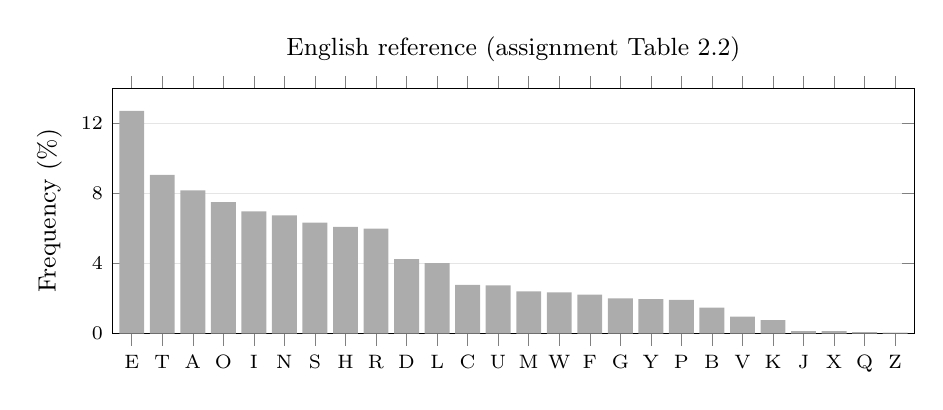
\begin{tikzpicture}
\begin{axis}[width=0.97\textwidth,height=4.7cm,ybar,bar width=9pt,ymin=0,ymax=14,ytick={0,4,8,12},ylabel={Frequency (\%)},symbolic x coords={E,T,A,O,I,N,S,H,R,D,L,C,U,M,W,F,G,Y,P,B,V,K,J,X,Q,Z},xtick=data,xticklabel style={font=\scriptsize},title={English reference (assignment Table 2.2)},title style={font=\small},tick label style={font=\scriptsize},label style={font=\small},ymajorgrids=true,grid style={gray!20},enlarge x limits=0.025]
\addplot[fill=gray!65,draw=none] coordinates {(E,12.7000) (T,9.0600) (A,8.1700) (O,7.5100) (I,6.9700) (N,6.7500) (S,6.3300) (H,6.0900) (R,5.9900) (D,4.2500) (L,4.0300) (C,2.7800) (U,2.7600) (M,2.4100) (W,2.3600) (F,2.2300) (G,2.0100) (Y,1.9700) (P,1.9300) (B,1.4900) (V,0.9800) (K,0.7700) (J,0.1500) (X,0.1500) (Q,0.0900) (Z,0.0700)};
\end{axis}
\end{tikzpicture}
\par\vspace{0.3cm}
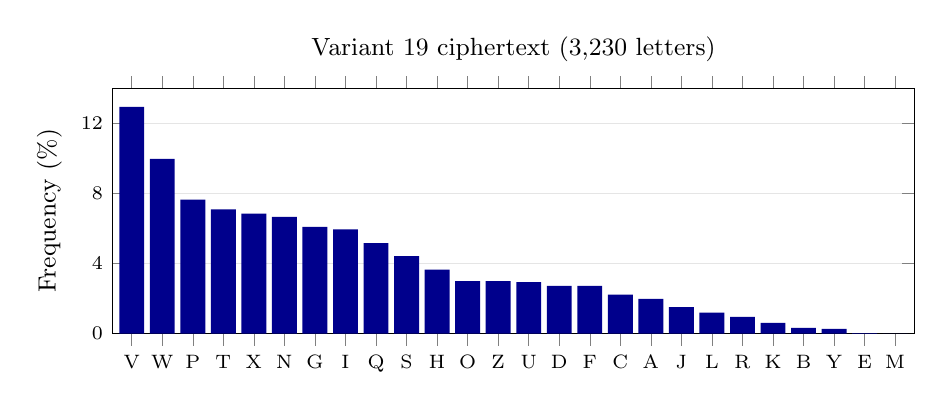
\begin{tikzpicture}
\begin{axis}[width=0.97\textwidth,height=4.7cm,ybar,bar width=9pt,ymin=0,ymax=14,ytick={0,4,8,12},ylabel={Frequency (\%)},symbolic x coords={V,W,P,T,X,N,G,I,Q,S,H,O,Z,U,D,F,C,A,J,L,R,K,B,Y,E,M},xtick=data,xticklabel style={font=\scriptsize},title={Variant 19 ciphertext (3,230 letters)},title style={font=\small},tick label style={font=\scriptsize},label style={font=\small},ymajorgrids=true,grid style={gray!20},enlarge x limits=0.025]
\addplot[fill=blue!55!black,draw=none] coordinates {(V,12.9412) (W,9.9690) (P,7.6471) (T,7.0898) (X,6.8421) (N,6.6563) (G,6.0991) (I,5.9443) (Q,5.1703) (S,4.4272) (H,3.6533) (O,3.0031) (Z,3.0031) (U,2.9412) (D,2.7245) (F,2.7245) (C,2.2291) (A,1.9814) (J,1.5170) (L,1.2074) (R,0.9598) (K,0.6192) (B,0.3406) (Y,0.2786) (E,0.0310) (M,0.0000)};
\end{axis}
\end{tikzpicture}

\caption{English reference and variant 19 frequencies, each independently sorted}
\label{fig:frequencies}\end{figure}

The two graphs show a similar overall frequency profile. Their horizontal
positions represent frequency rank, so vertically aligned bars are not
necessarily the same plaintext letter. Word and n-gram evidence is needed
to establish the actual correspondence.

The service's \textit{Count Digraphs}, \textit{Count Trigraphs} and
\textit{Count Doubles} options produced the combinations below. For the
counts shown in this report, combinations are counted within uninterrupted
runs of letters, without joining across spaces or punctuation. Missing
spaces already present in the copied variant are left intact.

\begin{table}[H]\caption{Most frequent letter combinations in variant 19}
\centering\small
\begin{tabular}{l p{0.70\textwidth}}\toprule
Type & Ciphertext combinations, in the service's order\\\midrule
Digraphs & \texttt{WQ, QV, VI, XG, IV, PW, NG, SV, XW, TG, QT, VP, VG}\\
Trigraphs & \texttt{WQV, QTW, WQT, ASV, VGW, XGJ, QVI, TGO, WXN, XNG, FPW, NDS, DSO}\\
Doubles & \texttt{SS, PP, WW, CC, VV, II, UU, NN, ZZ, HH, GG}\\\bottomrule
\end{tabular}\end{table}

\clearpage
\chapter{Step-by-step recovery of the substitution}
\section{The first seven substitutions from my working notes}
I started with the frequent trigram \texttt{WQV}, which occurs 63 times
inside letter runs and appears 44 times as a separate word. The English
word THE is a strong candidate. This also fits the frequent digraphs
\texttt{WQ} (91 occurrences) and \texttt{QV} (81 occurrences).

My recorded first substitution~\cite{ref:notes} was \pair{W}{T}. I then added
\pair{Q}{H} and \pair{V}{E}, one at a time, obtaining \texttt{the} from
\texttt{WQV}. The opening after these three substitutions is
\partialtext{03}

Next, \texttt{WQVPV} became \texttt{thePe}, which suggested THESE.
I replaced P with S, obtaining \texttt{these}. This was checked against
\texttt{PFPWVZ}, which became \texttt{sFsteZ}, a likely instance of SYSTEM.
The next substitution, \pair{F}{Y}, gave \texttt{systeZ}; it also changed
\texttt{LVF} into \texttt{LeY}, suggesting KEY. Replacing Z with M completed
\texttt{system}. Finally, I replaced T with A: \texttt{WQTW} became
\texttt{that}, and other partial words gained the expected A positions.

\begin{table}[H]\caption{Recorded order of the first seven substitutions}
\centering\small
\begin{tabular}{ccl}\toprule
Step & Substitution & Main evidence\\\midrule
1 & \pair{W}{T} & \texttt{WQV} is a candidate for THE\\
2 & \pair{Q}{H} & \texttt{tQV} becomes \texttt{thV}\\
3 & \pair{V}{E} & \texttt{thV} becomes \texttt{the}; V is the most frequent symbol\\
4 & \pair{P}{S} & \texttt{thePe} becomes \texttt{these}\\
5 & \pair{F}{Y} & \texttt{sFsteZ} becomes \texttt{systeZ}; \texttt{LeF} becomes \texttt{Ley}\\
6 & \pair{Z}{M} & \texttt{systeZ} becomes \texttt{system}\\
7 & \pair{T}{A} & \texttt{thTt} becomes \texttt{that}\\\bottomrule
\end{tabular}\end{table}

After these seven substitutions, the opening is
\partialtext{07}
The supplied working notes stop at \pair{T}{A}. The following sections
complete the analysis using the same word-pattern method; they present a
reproducible continuation rather than additional recorded dialogue.

\clearpage
\section{Recognising KEY, FROM, FOR, IN and AND}
The word \texttt{LVF} now reads \texttt{Ley}. In the repeated phrase
\texttt{the Ley}, KEY is the natural hypothesis, so I add \pair{L}{K}.
This is later checked in the longer phrase \textit{the specific key}.

The opening \texttt{CINm these tRN} suggests \textit{from these two}.
FROM gives \pair{C}{F}, \pair{I}{R} and \pair{N}{O}. The separate word
\texttt{CNI} then becomes \texttt{for}, and \texttt{NC} becomes
\texttt{of}, supporting all three assignments in several contexts.
\partialtext{11}

The short word \texttt{XW} now reads \texttt{Xt}. IT is a plausible match,
so I add \pair{X}{I}. The repeated pair \texttt{XG} becomes \texttt{iG},
suggesting IN and therefore \pair{G}{N}. This also makes
\texttt{GNW} read \texttt{not}. The frequent trigram \texttt{TGO}
now reads \texttt{anO}; AND supplies \pair{O}{D}.

These hypotheses are checked together, rather than accepted from one
isolated word: \texttt{XG}$\to$IN, \texttt{XW}$\to$IT,
\texttt{GNW}$\to$NOT and \texttt{TGO}$\to$AND all produce sensible
English in the surrounding sentences.

\section{Recovering SHOULD and BE}
With the previous substitutions, \texttt{PQNDSO} reads \texttt{shoDSd}.
The repeated construction \texttt{the system shoDSd Ae} strongly suggests
\textit{the system should be}. SHOULD gives \pair{D}{U} and \pair{S}{L};
BE gives \pair{A}{B}. The double \texttt{SS} becomes LL, which also fits
\texttt{TSS}$\to$ALL and the ending of FULFILLED.

At this point 17 cipher symbols have been recovered. The opening becomes
\partialtext{17}
The emerging words \texttt{fundamental}, \texttt{principles} and
\texttt{requirements} provide longer checks on the same assignments.

\clearpage
\section{Completing the technical vocabulary and rare letters}
The text repeatedly refers to ciphers and their keys. In that context,
\texttt{HIFUWNJITUQVI} is a candidate for CRYPTOGRAPHER. Its known letters
already fit, and it supplies \pair{H}{C}, \pair{U}{P} and \pair{J}{G}.
The same assignments are checked in \texttt{HXUQVI}$\to$CIPHER,
\texttt{UITHWXHV}$\to$PRACTICE and \texttt{HIFUWNJITZP}$\to$CRYPTOGRAMS.
The double \texttt{CC} becomes FF, supporting the repeated name
KERCKHOFFS after the rest of that name is completed.

The pattern \texttt{RQXHQ} now reads \texttt{Rhich}. WHICH gives
\pair{R}{W}. This also completes \texttt{WRN}$\to$TWO at the beginning
and \texttt{RXWQNDW}$\to$WITHOUT. The partial word
\texttt{QTKV} reads \texttt{haKe}; HAVE supplies \pair{K}{V}.
\partialtext{22}

Three observed symbols remain. \texttt{VYUSXHXW} reads \texttt{eYplicit},
which suggests EXPLICIT and gives \pair{Y}{X}. The word
\texttt{WVHQGXBDV} reads \texttt{techniBue}, so TECHNIQUE gives
\pair{B}{Q}. Finally, the phrase containing \texttt{WNHNGEDIV}
reads \texttt{toconEure}; restoring the word boundary gives
\textit{to conjure}, so \pair{E}{J}. E occurs only once, which explains
why frequency ranking alone was insufficient to recover J.
\partialtext{25}

The entire passage is now readable. These final substitutions are checked
in the full message, including EXCEPTIONS, REQUIREMENTS and CONJURE.
A readable result everywhere is stronger evidence than a plausible
replacement in just one short word.

\section{Completing the alphabet and checking consistency}
All 25 symbols that occur in the message now have a consistent plaintext
letter. The cipher symbol M has count zero. Under the assumption that the
cipher uses a permutation of all 26 English letters, the only unused
plaintext letter is Z; hence \pair{M}{Z} follows by elimination. This pair
is inferred from alphabet completion and is not directly observed in V19.
It has no effect on decoding this message.

The frequent patterns now have the following meanings:
\texttt{WQ}$\to$TH, \texttt{QV}$\to$HE, \texttt{WQV}$\to$THE,
\texttt{QTW}$\to$HAT, \texttt{WQT}$\to$THA, \texttt{TGO}$\to$AND,
\texttt{ASV}$\to$BLE and \texttt{XGJ}$\to$ING.
The doubles become LL, SS, TT, FF, EE, RR, PP, OO, MM, CC and NN.
These are consistent with the words in the recovered English passage.

\clearpage
\chapter{Recovered key and results}
\section{The substitution alphabets}
Table~\ref{tab:key} lists the decryption key: the upper row is the cipher
alphabet and the lower row is the corresponding plaintext alphabet.
All 26 output letters are distinct.
\begin{table}[H]\caption{Recovered decryption mapping, cipher letter to plaintext letter}
\label{tab:key}\centering\small
\setlength{\tabcolsep}{7pt}
\begin{tabular}{l*{13}{c}}\toprule
Cipher & A & B & C & D & E & F & G & H & I & J & K & L & M\\
Plain & B & Q & F & U & J & Y & N & C & R & G & V & K & Z$^{*}$\\\midrule
Cipher & N & O & P & Q & R & S & T & U & V & W & X & Y & Z\\
Plain & O & D & S & H & W & L & A & P & E & T & I & X & M\\\bottomrule
\end{tabular}\end{table}
\noindent\small $^{*}$M$\to$Z is inferred by elimination because M does not occur.\normalsize

For re-encryption, the inverse mapping is
\begin{center}\small\ttfamily
Plain: ABCDEFGHIJKLMNOPQRSTUVWXYZ\\
Cipher: TAHOVCJQXELSZGNUBIPWDKRYFM
\end{center}

The key was also entered into the online service and applied with
\textit{Make Substitutions}. The site's complete output agrees with the
independently checked decryption. Figure~\ref{fig:analyzer} shows the
opening of the recovered message and the filled substitution row.
\begin{figure}[H]\centering
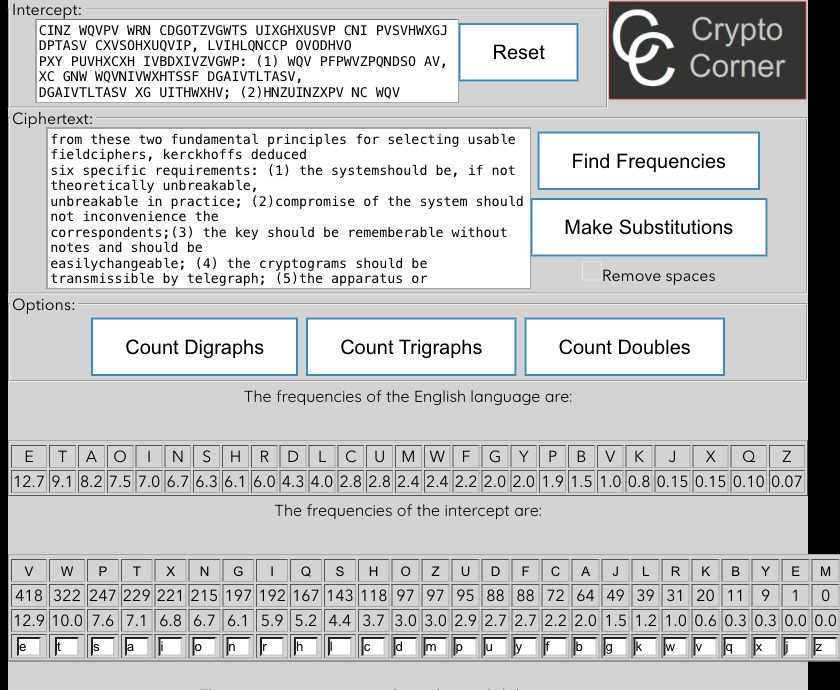
\includegraphics[width=0.84\textwidth]{img/analyzer_solution.png}
\caption{Variant 19 decoded in the frequency-analysis service}
\label{fig:analyzer}\end{figure}

\section{Verification and interpretation}
The mapping is one-to-one, all 25 observed symbols are decoded, and the
English text is coherent. Applying the inverse key reproduces the working
ciphertext exactly, including punctuation, digits, spaces and line breaks.
The original supplied paste is also reproduced exactly when its extraction
artifacts are retained.

The passage discusses Kerckhoffs' six requirements, the distinction between
a public system and a secret key, and superimposition of polyalphabetic
messages. These are topics in the recovered text; the attacked cipher is
monoalphabetic.

The PDF paste has merged words, a control separator in POST-TELEGRAPH and
a trailing backslash. The working input displays the separator as a hyphen
and excludes that backslash; the supplied version is retained separately.
The readable plaintext restores spacing, paragraphs and capitalization,
and omits the stray hyphen in \textit{have -been made}. All 3,230 letters
remain identical to the exact decryption. Exact forms are saved in
\texttt{data/plaintext\_exact.txt} and
\texttt{data/plaintext\_supplied\_exact.txt}.

\clearpage
\section{Complete recovered plaintext}
From these two fundamental principles for selecting usable field ciphers, Kerckhoffs deduced six specific requirements: (1) the system should be, if not theoretically unbreakable, unbreakable in practice; (2) compromise of the system should not inconvenience the correspondents; (3) the key should be rememberable without notes and should be easily changeable; (4) the cryptograms should be transmissible by telegraph; (5) the apparatus or documents should be portable and operable by a single person; (6) the system should be easy, neither requiring knowledge of a long list of rules nor involving mental strain.

These requirements still comprise the ideal which military ciphers aim at. They have been rephrased, and qualities that lie implicit have been made explicit. But any modern cryptographer would be very happy if any cipher fulfilled all six. Of course, it has never been possible to do that. There appears to be a certain incompatibility among them that makes it impossible to institute all of them at once. The requirement that is usually sacrificed is the first.

Kerckhoffs argued strongly against the notion of a field cipher that would simply resist solution long enough for the orders it transmitted to be carried out. This was not enough, he said, declaring that "the secret matter in communications sent over a distance very often retains its importance beyond the day on which it was transmitted." He was on the side of the angels, but a practical field cipher that is unbreakable was not possible in his day, nor is it today, and so military cryptography has settled for field ciphers that delay but do not defeat cryptanalysis.

Perhaps the most startling requirement, at first glance, was the second. Kerckhoffs explained that by "system" he meant "the material part of the system; tableaux, code books, or whatever mechanical apparatus may be necessary," and not "the key proper." Kerckhoffs here makes for the first time the distinction, now basic to cryptology, between the general system and the specific key. Why must the general system "not require secrecy," as, for example, a codebook requires it? Why must it be "a process that. . . our neighbors can even copy and adopt"?

Because, Kerckhoffs said, "it is not necessary to conjure up imaginary phantoms and to suspect the incorruptibility of employees or subalterns to understand that, if a system requiring secrecy were in the hands of too large a number of individuals, it could be compromised at each engagement in which one or another of them took part." This has proved to be true, and Kerckhoffs' second requirement has become widely accepted under a form that is sometimes called the fundamental assumption of military cryptography: that the enemy knows the general system. But he must still be unable to solve messages in it without knowing the specific key. In its modern formulation, the Kerckhoffs doctrine states that secrecy must reside solely in the keys.

Had Kerckhoffs merely published his perceptions of the problems facing post-telegraph cryptography and his prescriptions for resolving them, he would have assured a place for himself in the pantheon of cryptology. But he did more. He contributed a technique of cryptanalysis that is of supreme importance today. Called "superimposition," it constitutes the most general solution for polyalphabetic substitution systems. With few exceptions, it lays no restrictions on the type or length of keys, as does the Kasiski method, nor on the alphabets, which may be interrelated or entirely independent. It wants only several messages in the same key.

The cryptanalyst must align these one above the other so that letters enciphered with the same keyletter will fall into a single column. In the simplest case, that of a running key (a very long continuous text used as a key, as a novel) that restarts with each message, he can do this simply by placing all the first letters in the first column, all the second letters in the next column, and so on.


\clearpage
\chapter{Conclusions}
I recovered the plaintext of variant 19 through frequency analysis and
successive letter substitutions. The first seven recorded replacements
established THE, THESE, SYSTEM and THAT. Continuing with short words,
double letters and the emerging technical vocabulary allowed the remaining
observed letters to be identified. The full substitution was consistent
throughout the passage and reproduced the ciphertext when reversed.

The work demonstrates that letter frequencies are useful starting points,
but they do not determine the key on their own. For example, the third-most
frequent cipher symbol P represents S, while the rare symbol E represents
J. Digraphs, trigraphs, word patterns and sentence meaning supplied the
additional evidence needed to confirm these mappings.

I also learned to distinguish an observed substitution from one inferred
only by elimination: M does not appear in the ciphertext, so M$\to$Z
completes the assumed alphabet permutation without being directly tested
by the message. Preserving the exact input and decrypted versions makes
it possible to separate cryptographic correctness from corrections to
copied spacing and formatting.

Although monoalphabetic substitution has a large theoretical key space,
it preserves enough language structure to be vulnerable to this attack.
The main skills developed in this laboratory work were comparing
frequency distributions, testing hypotheses across several words,
maintaining a consistent substitution table and verifying a recovered
plaintext. No laboratory program was required.


\clearpage
\appendix
\chapter{Complete working ciphertext}
The following is the full V19 input used for the frequency analysis.
Capitalization and the copied word boundaries are preserved. The extraction
separator is displayed as a hyphen and the trailing paste backslash is
excluded, as explained in the verification section.
{\setstretch{1}\lstinputlisting[style=ciphertext,basicstyle=\ttfamily\fontsize{9}{10}\selectfont]{data/ciphertext.txt}}

\clearpage
\phantomsection
\addcontentsline{toc}{chapter}{Bibliography}
\begin{thebibliography}{9}
\singlespace\normalsize
\bibitem{ref:assignment}
Technical University of Moldova.
\textit{Lucrare de laborator nr. 2: Criptanaliza cifrurilor monoalfabetice}.
Course assignment, Sections 2.1--2.3 and variant V19, pp.~24--25.

\bibitem{ref:tool}
Crypto Corner. \textit{Frequency Analysis: Breaking the Code}.
Frequency-analysis and substitution activity specified by the assignment.
Accessed October 14, 2026.
\url{https://crypto.interactive-maths.com/frequency-analysis-breaking-the-code.html}.

\bibitem{ref:notes}
Pancenco, Mihail. \textit{Variant 19 working notes}.
Supplied ciphertext, frequency results and the recorded sequence of the
first seven substitutions.
\end{thebibliography}

\end{document}
